\documentclass[10pt]{beamer}
\usetheme{Goettingen}

\usepackage{amssymb, amsmath, amsfonts}
\usepackage{moreverb}
\usepackage{graphicx}
\usepackage{enumerate}
\usepackage{graphics}
\usepackage{color}
\usepackage{array}
\usepackage{float}
\usepackage{hyperref}
\usepackage{textcomp}
\usepackage{alltt}
\usepackage{mathtools}
\usepackage{tikz}
\usepackage{bigints}

\newcommand{\suchthat}{\, \mid \,}
\renewcommand{\theenumi}{\alph{enumi}}
\setcounter{section}{-1}
%\setlength{\jot}{30pt}

\title{The Ecological Effects of Trait Variation in a $u$-Predator, $v$-Prey System}
\author{Sam Fleischer, Pablo Chavarria}
\date{March 14, 2015}

\begin{document}

\begin{frame}
	\titlepage
\end{frame}

\section{Introduction}
\begin{frame}
	\frametitle{}
	{\bf Advisors}
	\begin{itemize}
		\item Dr. Jing Li \\
		Assistant Professor, CSU Northridge \\
		Department of Mathematics
		\item Dr. Casey terHorst \\
		Assistant Professor, CSU Northridge \\
		Biology Department
	\end{itemize}
	{\bf Funding}
	\begin{itemize}
		\item National Science Foundation \\
		Pacific Math Alliance \\
		Preparing Undergraduates through Mentoring towards PhDs (PUMP)
	\end{itemize}
\end{frame}

\section{Motivation}
\begin{frame}
	\frametitle{}
	{\bf Observations}
	\begin{itemize}
		\item Predator/Prey interactions are prevalent in nature
		\begin{itemize}
			\item Crab vs. gastropod
			\item Protist vs. bacteria
		\end{itemize}
		\item There is trait variation within species
		\begin{itemize}
			\item Thickness of plant cuticula
			\item Strength of gastropod shell
		\end{itemize}
		\item Incorporating trait variation provides richer dynamics than classical Lotka-Volterra models
	\end{itemize}
\end{frame}

\section{Model Formulation}
\subsection{Lotka-Volterra}
\begin{frame}
	\begin{align*}
		\frac{dN}{dt} &= N(b - aM)\\[.1cm]
		\frac{dM}{dt} &= M(eaN - d)
	\end{align*}
	{\bf Variables}
	\begin{itemize}
		\item $N \equiv $ Prey Density
		\item $M \equiv $ Predator Density
	\end{itemize}
	{\bf Parameters}
	\begin{itemize}
		\item $a \equiv $ Attack rate \uncover<2->{\ \ \ \ \ $\longleftarrow$ {\it No variation!}}
		\item $b \equiv $ Prey birth rate
		\item $e \equiv $ Efficiency
		\item $d \equiv $ Predator death rate
	\end{itemize}
\end{frame}
\subsection{Schreiber, B\"urger, and Bolnick}
\begin{frame}
	\begin{align*}
		a(m) = \alpha \exp\left[-\frac{(m - \theta)^2}{2\tau^2}\right]
	\end{align*}
	{\bf Variables}
	\begin{itemize}
		\item $N \equiv $ Prey Density
		\item $M \equiv $ Predator Density
		\item $m \equiv $ Predator Character (Trait Value)
	\end{itemize}
	{\bf Parameters}
	\begin{itemize}
		\item $\alpha \equiv $ Maximum attack rate
		\item $\theta \equiv $ Optimal trait value \uncover<2->{\ \ \ \ \ $\longleftarrow$ {\it No variation!}}
		\item $\tau \equiv $ Specialization Constant
	\end{itemize}
\end{frame}
\subsection{Our Extension}
\begin{frame}
	\begin{align*}
		a(m, n) = \alpha \exp\left[-\frac{(m - n - \theta)^2}{2\tau^2}\right]
	\end{align*}
	{\bf Variables}
	\begin{itemize}
		\item $N \equiv $ Prey Density
		\item $M \equiv $ Predator Density
		\item $n \equiv $ Prey Character (Trait Value)
		\item $m \equiv $ Predator Character (Trait Value)
	\end{itemize}
	{\bf Parameters}
	\begin{itemize}
		\item $\alpha \equiv $ Maximum attack rate
		\item $\theta \equiv $ Optimal trait {\it difference}
		\item $\tau \equiv $ Specialization Constant
	\end{itemize}
\end{frame}
\begin{frame}
	\frametitle{}
	{\bf Distribution Assumptions}
	\begin{itemize}
		\item Trait values are {\bf normally distributed} over the populations
	\end{itemize}
	\begin{align*}
		p(n, \overline{n}) &= \frac{1}{\sqrt{2\pi\beta^2}}\exp\left[{-\frac{(n - \overline{n})^2}{2\beta^2}}\right] \\
		p(m, \overline{m}) &= \frac{1}{\sqrt{2\pi\sigma^2}}\exp\left[{-\frac{(m - \overline{m})^2}{2\sigma^2}}\right]
	\end{align*}
	{\bf Variables}
	\begin{itemize}
		\item $N \equiv $ Prey Density
		\item $\overline{n} \equiv $ Mean Prey Character
		\item $M \equiv $ Predator Density
		\item $\overline{m} \equiv $ Mean Predator Character
	\end{itemize}
	{\bf Parameters}
	\begin{itemize}
		\item $\beta^2 \equiv $ Prey Trait Variance
		\item $\sigma^2 \equiv $ Predator Trait Variance
	\end{itemize}
\end{frame}
\begin{frame}
	\frametitle{}
	{\bf Average Attack Rate}
	\begin{align*}
		\overline{a}(\overline{m}, \overline{n}) &= \int_{-\infty}^{\infty}\int_{\-\infty}^{\infty} a_{}(m, n) \cdot p(m, \overline{m}) \cdot p(n, \overline{n}) dm dn \\
		&= \frac{\alpha\tau}{\sqrt{\sigma^2 + \beta^2 + \tau^2}}\exp\left[{-\frac{(\overline{m} - \overline{n} - \theta)^2}{2(\sigma^2 + \beta^2 + \tau^2)}}\right]
	\end{align*}
	{\bf Variables}
	\begin{itemize}
		\item $N \equiv $ Prey Density
		\item $\overline{n} \equiv $ Mean Prey Character
		\item $M \equiv $ Predator Density
		\item $\overline{m} \equiv $ Mean Predator Character
	\end{itemize}
	{\bf Parameters}
	\begin{itemize}
		\item $\beta^2 \equiv $ Prey Trait Variance
		\item $\sigma^2 \equiv $ Predator Trait Variance
		\item $\alpha \equiv $ Maximum attack rate
		\item $\theta \equiv $ {\it Optimal trait difference}
		\item $\tau \equiv $ Specialization Constant
	\end{itemize}
\end{frame}
\begin{frame}
	\frametitle{}
	{\bf Fitness Assumptions}
	\begin{itemize}
		\item Prey experiences logistic growth in absence of predator
		\item Predator experiences exponential decay in absence of prey
	\end{itemize}
	\begin{align*}
		Y(m, n, M, N) &= r\left(1 - \frac{N}{K}\right) - Ma(m, n) \\[.1cm]
		W(m, n, N) &= eNa(m, n) - d
	\end{align*}
	{\bf Variables}
	\begin{itemize}
		\item $N \equiv $ Prey Density
		\item $n \equiv $ Prey Character
		\item $M \equiv $ Predator Density
		\item $m \equiv $ Predator Character
	\end{itemize}
	{\bf Parameters}
	\begin{itemize}
		\item $r \equiv $ Intrinsic Prey Growth Rate
		\item $K \equiv $ Prey Carrying Capacity
		\item $d \equiv $ Predator Death Rate
		\item $e \equiv $ Efficiency
	\end{itemize}
\end{frame}
\begin{frame}
	\frametitle{}
	{\bf Average Fitness}
	\begin{align*}
	\overline{Y}(\overline{m}, \overline{n}, M, N) &= \int_{-\infty}^{\infty}\int_{-\infty}^{\infty} Y(m, n, M, N) \cdot p(m, \overline{m}) \cdot p(n, \overline{n}) dm dn \\
	&= r\left(1 - \frac{N}{K}\right) - M\overline{a}(\overline{m}, \overline{n}) \\[.1cm]
	\overline{W}(\overline{m}, \overline{n}, N) &= \int_{-\infty}^{\infty}\int_{-\infty}^{\infty} W(m, n, N) \cdot p(m, \overline{m}) \cdot p(n, \overline{n}) dm dn \\
	&= eN\overline{a}(\overline{m}, \overline{n}) - d
	\end{align*}
	{\bf Variables}
	\begin{itemize}
		\item $N \equiv $ Prey Density
		\item $\overline{n} \equiv $ Mean Prey Character
		\item $M \equiv $ Predator Density
		\item $\overline{m} \equiv $ Mean Predator Character
	\end{itemize}
	{\bf Parameters}
	\begin{itemize}
		\item $r \equiv $ Intrinsic Prey Growth Rate
		\item $K \equiv $ Prey Carrying Capacity
		\item $d \equiv $ Predator Death Rate
		\item $e \equiv $ Efficiency
	\end{itemize}
\end{frame}
\begin{frame}
	\frametitle{}
	{\bf Ecological Components}
	\begin{align*}
		\frac{dN}{dt} &= N\cdot \overline{Y}(\overline{m}, \overline{n}, M, N)\\[.1cm]
		\frac{dM}{dt} &= M\cdot \overline{W}(\overline{m}, \overline{n}, N)
	\end{align*}
	{\bf Variables}
	\begin{itemize}
		\item $N \equiv $ Prey Density
		\item $\overline{n} \equiv $ Mean Prey Character
		\item $M \equiv $ Predator Density
		\item $\overline{m} \equiv $ Mean Predator Character
	\end{itemize}
	{\bf Parameters}
	\begin{itemize}
		\item $r \equiv $ Intrinsic Prey Growth Rate
		\item $K \equiv $ Prey Carrying Capacity
		\item $d \equiv $ Predator Death Rate
		\item $e \equiv $ Efficiency
	\end{itemize}
\end{frame}
\begin{frame}
	\frametitle{}
	{\bf Evolutionary Components}
	\begin{itemize}
		\item The evolution of the mean character is always in the direction which increases the mean fitness in the population.
	\end{itemize}
	\begin{align*}
	\frac{d\overline{n}}{dt} &= \beta_G^2\frac{\partial \overline{Y}}{\partial \overline{n}}\\[.1cm]
	\frac{d\overline{m}}{dt} &= \sigma_G^2\frac{\partial \overline{W}}{\partial \overline{m}}\\
	\end{align*}
	{\bf Variables}
	\begin{itemize}
		\item $N \equiv $ Prey Density
		\item $\overline{n} \equiv $ Mean Prey Character
		\item $M \equiv $ Predator Density
		\item $\overline{m} \equiv $ Mean Predator Character
	\end{itemize}
	{\bf Parameters}
	\begin{itemize}
		\item $\beta_G^2 \equiv $ Prey genetic variance
		\item $\sigma_G^2 \equiv $ Predator genetic variance
	\end{itemize}
\end{frame}
\begin{frame}
	\frametitle{The Complete $1\times1$ Model \\ (One Predator Species, One Prey Species)}
	{\bf Ecological Components}
	\begin{align*}
	\frac{dN}{dt} &= N\cdot \overline{Y}(\overline{m}, \overline{n}, M, N)\ \ =\ N\left[r\left(1 - \frac{N}{K}\right) - M\overline{a}(\overline{m}, \overline{n})\right]\\[.1cm]
	\frac{dM}{dt} &= M\cdot \overline{W}(\overline{m}, \overline{n}, N)\ \ \ \ \ =\ M\left[eN\overline{a}(\overline{m}, \overline{n}) - d\right]
	\end{align*}
	{\bf Evolutionary Components}
	\begin{align*}
	\frac{d\overline{n}}{dt} &= \beta_G^2\frac{\partial \overline{Y}}{\partial \overline{n}} = \beta_G^2\frac{M(\theta + \overline{n} - \overline{m})}{\sigma^2 + \beta^2 + \tau^2} \overline{a}(\overline{m}, \overline{n})\\[.1cm]
	\frac{d\overline{m}}{dt} &= \sigma_G^2\frac{\partial \overline{W}}{\partial \overline{m}} = \sigma_G^2\frac{eN(\theta + \overline{n} - \overline{m})}{\sigma^2 + \beta^2 + \tau^2} \overline{a}(\overline{m}, \overline{n})
	\end{align*}
\end{frame}
\begin{frame}
	\frametitle{}
	{\bf Prey Fitness}
	\begin{align*}
		Y(m, n, M, N) &= r\left(1 - \frac{N}{K}\right) - Ma(m, n) \\
		\uncover<2->{&\downarrow} \\
		\uncover<2->{Y_j([m_i]_{i=1}^{u}, n_j, [M_i]_{i=1}^{u}, N_j) &= r_j\left(1 - \frac{N_j}{K_j}\right) - \sum\limits_{i = 1}^{u}M_ia_{ij}(m_i, n_j)}
	\end{align*}
	{\bf Predator Fitness}
	\begin{align*}
		W(m, n, N) &= eNa(m, n) - d \\
		\uncover<3->{&\downarrow} \\
		\uncover<3->{W_i(m_i, [n_j]_{j=1}^{v}, [N_j]_{j=1}^{v}) &= \sum\limits_{j = 1}^{v}\Big[e_{ij}N_ja_{ij}(m_i, n_j)\Big] - d_i}
	\end{align*}
	\uncover<2->{{\bf Notation}}
	\begin{align*}
		\uncover<2->{[x_i]_{i=1}^{u} = x_1, \dots, x_u}
	\end{align*}
\end{frame}
\begin{frame}
	\frametitle{}
	{\bf Average Fitness}
	\begin{align*}
		\overline{Y}_j([\overline{m}_i]_{i=1}^{u}, \overline{n}_j,\ &[M_i]_{i=1}^{u}, N_j) \\
		&= \int\limits_{\mathbb{R}^{u+1}} Y_j \cdot \prod\limits_{i=1}^{u}\Big[p_i(m_i, \overline{m_i})\Big] \cdot p(n, \overline{n}) \prod\limits_{i=1}^{u}\Big[dm_i\Big] dn_j\\
		&= r_j\left(1 - \frac{N_j}{K_j}\right) - \sum\limits_{i = 1}^{u}M_i\overline{a}_{ij}(\overline{m}_i, \overline{n}_j)
	\end{align*}
	\begin{align*}
		\overline{W}_i(\overline{m}_i, [\overline{n}_j]_{j=1}^{v}, [&N_j]_{j=1}^{v}) \\
		&= \int\limits_{\mathbb{R}^{u+1}} W_i \cdot p_i(m_i, \overline{m_i}) \cdot \prod\limits_{j=1}^{v}\Big[p(n_j, \overline{n}_j)\Big] dm_i \prod\limits_{j=1}^{v}\Big[dn_j\Big]\\
		&= \sum\limits_{j = 1}^{v}\Big[e_{ij}N_j\overline{a}_{ij}(\overline{m}_i, \overline{n}_j)\Big] - d_i
	\end{align*}
\end{frame}
\begin{frame}
	\frametitle{The Complete $u\times v$ Model \\ ($u$ Predator Species, $v$ Prey Species)}
	{\bf Ecological Components}
	\begin{align*}
		\frac{dN_j}{dt} &= N_j\overline{Y}_j = N_j \left[r_j\left(1 - \frac{N_j}{K_j}\right) - \sum\limits_{i = 1}^{u}M_i\overline{a}_{ij}(\overline{m}_i, \overline{n}_j)\right] \\[.1cm]
		\frac{dM_i}{dt} &= M_i\overline{W}_i = M_i \left[\sum\limits_{j = 1}^{v}\Big[e_{ij}N_j\overline{a}_{ij}(\overline{m}_i, \overline{n}_j)\Big] - d_i\right]
	\end{align*}
	{\bf Evolutionary Components}
	\begin{align*}
	\frac{d\overline{n}_j}{dt} &= \beta_{jG}^2\frac{\partial \overline{Y}_j}{\partial \overline{n}_j} = \beta_{jG}^2\sum\limits_{i=1}^{u}\left[\frac{M_i(\theta_{ij} + \overline{n_j} - \overline{m_i})}{\sigma_i^2 + \beta_j^2 + \tau_{ij}^2} \overline{a}_{ij}(\overline{m_i}, \overline{n_j})\right]\\[.1cm]
	\frac{d\overline{m}_i}{dt} &= \sigma_{iG}^2\frac{\partial \overline{W}_i}{\partial \overline{m}_i} = \sigma_{iG}^2\sum\limits_{j=1}^{v}\left[\frac{e_{ij}N_j(\theta_{ij} + \overline{n_j} - \overline{m_i})}{\sigma_i^2 + \beta_j^2 + \tau_{ij}^2} \overline{a}_{ij}(\overline{m_i}, \overline{n_j})\right]
	\end{align*}
\end{frame}

\section{Preliminary Results}
\subsection{$1 \times 1$}
\begin{frame}
	\frametitle{Equilibria}
	\begin{align*}
		\begin{array}{ll}
			\dfrac{dN}{dt} = N\cdot \overline{Y}(\overline{m}, \overline{n}, M, N) &\ \ \ \ \ \ \dfrac{d\overline{n}}{dt} = \beta_G^2\dfrac{\partial \overline{Y}}{\partial \overline{n}} \\[.3cm]
			\dfrac{dM}{dt} = M\cdot \overline{W}(\overline{m}, \overline{n}, N) & \ \ \ \ \ \ \dfrac{d\overline{m}}{dt} = \sigma_G^2\dfrac{\partial \overline{W}}{\partial \overline{m}}
		\end{array}
	\end{align*}
	{\bf Extinction} \uncover<2->{$\boxed{\text{\it Unstable}}$}
	\begin{align*}
		(N^*, M^*, \overline{n}^*, \overline{m}^*) = (0, 0, \underline{\ \ }, \underline{\ \ })
	\end{align*}
	{\bf Exclusion} \uncover<3->{$\boxed{\text{\it Stable under certain conditions}}$}
	\begin{align*}
		(N^*, M^*, \overline{n}^*, \overline{m}^*) = (K, 0, \underline{\ \ }, \underline{\ \ })
	\end{align*}
	\uncover<4->{{\bf Necessary Conditions for Stable Exclusion:}}
	\begin{itemize}
		\item \uncover<4->{$d > e\overline{a}(\overline{m}^*, \overline{n}^*)K$}
		\item \uncover<4->{$(\overline{m}^* - \overline{n}^* - \theta)^2 < \sigma^2 + \beta^2 + \tau^2$}
	\end{itemize}
\end{frame}
\begin{frame}
	\frametitle{Equilibria}
	\begin{align*}
		\begin{array}{ll}
			\dfrac{dN}{dt} = N\cdot \overline{Y}(\overline{m}, \overline{n}, M, N) &\ \ \ \ \ \ \dfrac{d\overline{n}}{dt} = \beta_G^2\dfrac{\partial \overline{Y}}{\partial \overline{n}} \\[.3cm]
			\dfrac{dM}{dt} = M\cdot \overline{W}(\overline{m}, \overline{n}, N) & \ \ \ \ \ \ \dfrac{d\overline{m}}{dt} = \sigma_G^2\dfrac{\partial \overline{W}}{\partial \overline{m}}
		\end{array}
	\end{align*}
	{\bf Coexistence} \uncover<2->{$\boxed{\text{\it Stable under certain conditions}}$}
	\begin{align*}
		(N^*, M^*, \overline{n}^*, \overline{m}^*) = (\dfrac{d\sqrt{A}}{e \alpha \tau}\ ,\ \dfrac{r\sqrt{A}}{\alpha\tau}\left(1 - \dfrac{d\sqrt{A}}{Ke\alpha\tau}\right)\ ,\ \mu^*\ ,\ \mu^* - \theta) \\[.1cm]
		\text{where $A = \sigma^2 + \beta^2 + \tau^2$ and $\mu^*$ is an arbitrary value.}
	\end{align*}
	\uncover<3->{{\bf Necessary Condition for Stable Coexistence:}}
	\begin{itemize}
		\item \uncover<3->{$d\sigma_G^2 > r\beta_G^2\left(1 - \dfrac{d\sqrt{A}}{Ke\alpha\tau}\right)$}
	\end{itemize}
\end{frame}
\begin{frame}
	\frametitle{Figures}
	{\bf Exclusion}
	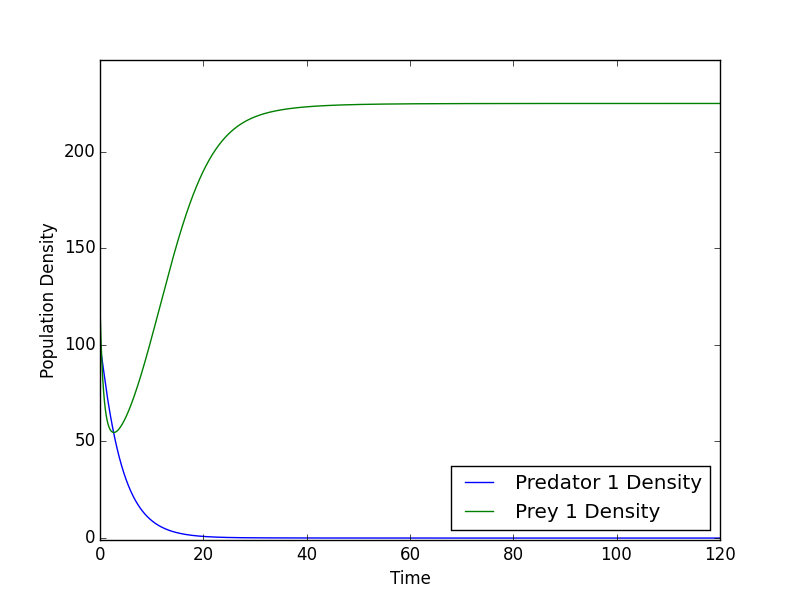
\includegraphics[scale=0.5]{figures/1x1/densities_exclusion.png}
\end{frame}
\begin{frame}
	\frametitle{Figures}
	{\bf Exclusion}
	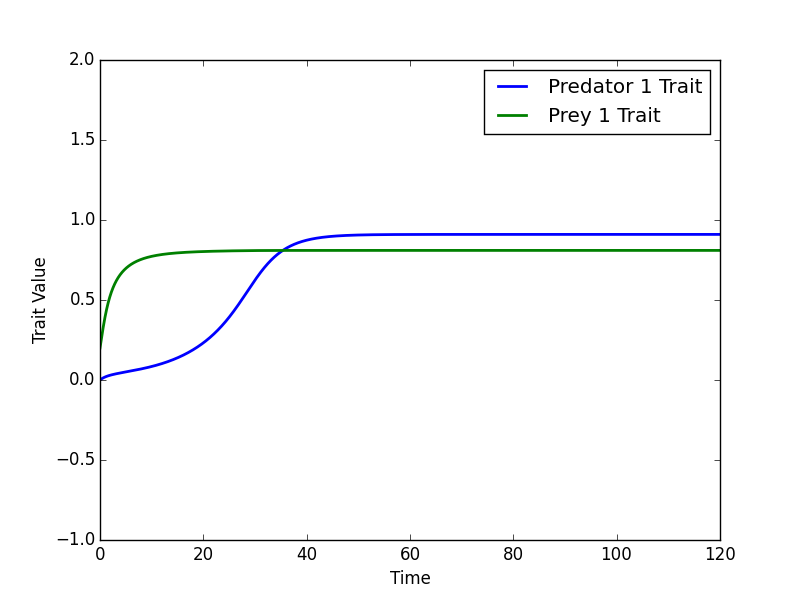
\includegraphics[scale=0.5]{figures/1x1/traits_exclusion.png}
\end{frame}
\begin{frame}
	\frametitle{Figures}
	{\bf Stable Coexistence}
	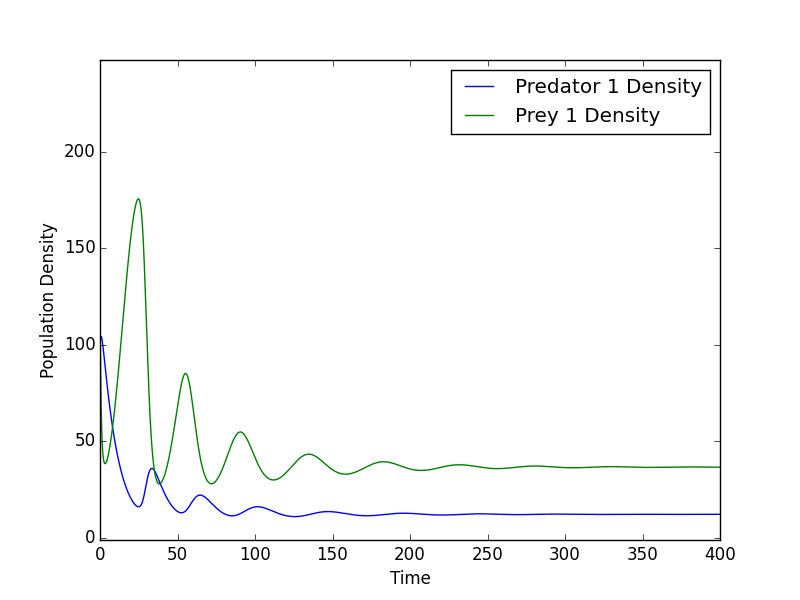
\includegraphics[scale=0.5]{figures/1x1/densities_stable_coexistence.png}
\end{frame}
\begin{frame}
	\frametitle{Figures}
	{\bf Stable Coexistence}
	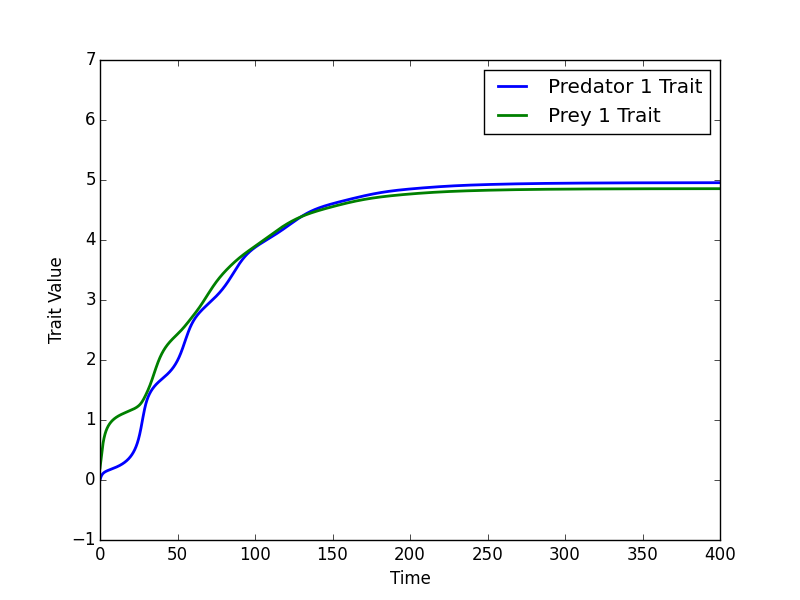
\includegraphics[scale=0.5]{figures/1x1/traits_stable_coexistence.png}
\end{frame}
\begin{frame}
	\frametitle{Figures}
	{\bf Unstable Coexistence}
	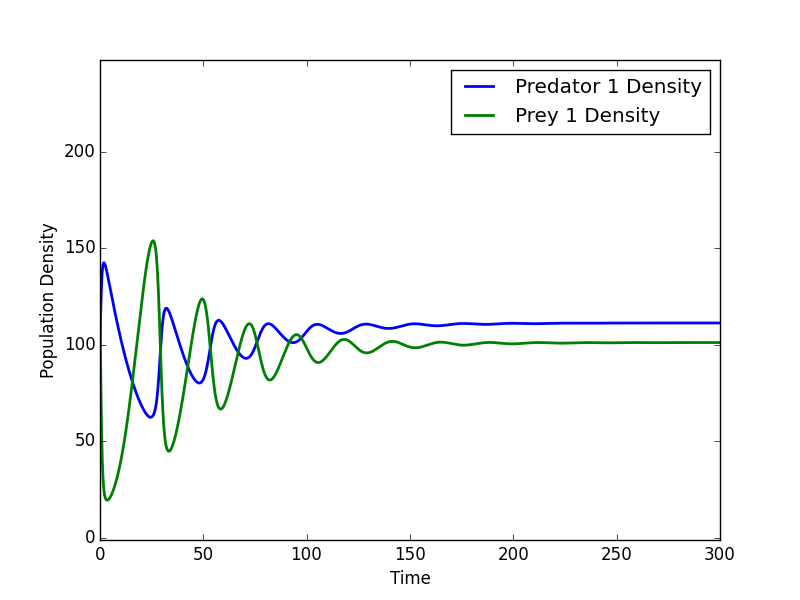
\includegraphics[scale=0.5]{figures/1x1/densities_unstable_coexistence.png}
\end{frame}
\begin{frame}
	\frametitle{Figures}
	{\bf Unstable Coexistence}
	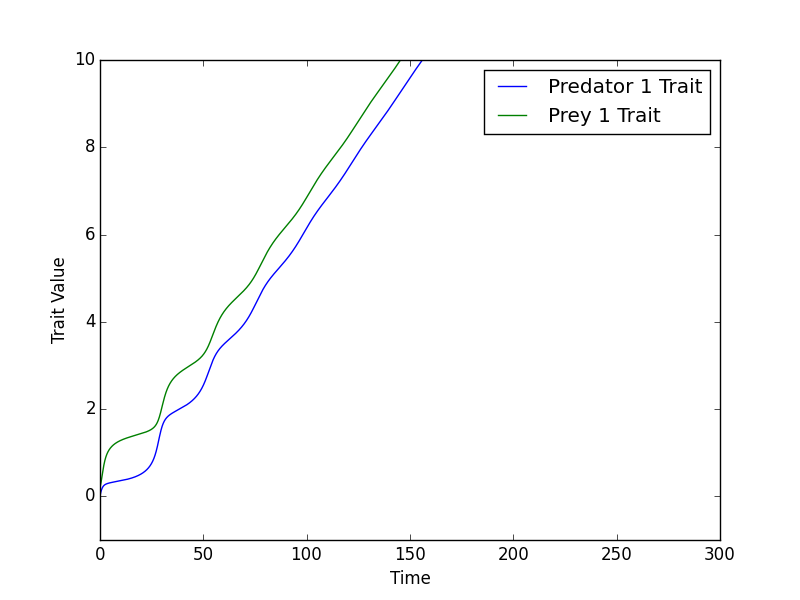
\includegraphics[scale=0.5]{figures/1x1/traits_unstable_coexistence.png}
\end{frame}

\subsection{$1 \times 2$}
\begin{frame}
	\frametitle{Equilibria}
	\begin{align*}
		\begin{array}{ll}
			\dfrac{dN_1}{dt} = N_1\cdot \overline{Y}_1(\overline{m}, \overline{n}_1, M, N_1) &\ \ \ \ \ \ \dfrac{d\overline{n}_1}{dt} = \beta_{1,G}^2\dfrac{\partial \overline{Y}_1}{\partial \overline{n}_1} \\[.3cm]
			\dfrac{dN_2}{dt} = N_2\cdot \overline{Y}_2(\overline{m}, \overline{n}_2, M, N_2) &\ \ \ \ \ \ \dfrac{d\overline{n}_2}{dt} = \beta_{2,G}^2\dfrac{\partial \overline{Y}_2}{\partial \overline{n}_2} \\[.3cm]
			\dfrac{dM}{dt} = M\cdot \overline{W}(\overline{m}, \overline{n}_1, \overline{n}_2, N_1, N_2) & \ \ \ \ \ \ \dfrac{d\overline{m}}{dt} = \sigma_G^2\dfrac{\partial \overline{W}}{\partial \overline{m}}
		\end{array}
	\end{align*}
	\uncover<2->{{\bf Extinction}} \uncover<3->{$\boxed{\text{\it Unstable}}$}
	\begin{align*}
		\uncover<2->{(N_1^*, N_2^*, M^*, \overline{n}_1^*, \overline{n}_2^*, \overline{m}^*) = (0, 0, 0, \underline{\ \ }, \underline{\ \ }, \underline{\ \ })}
	\end{align*}
	\uncover<4->{{\bf Exclusion}} \uncover<5->{$\boxed{\text{\it Stable under certain conditions}}$}
	\begin{align*}
		\uncover<4->{(N_1^*, N_2^*, M^*, \overline{n}_1^*, \overline{n}_2^*, \overline{m}^*) &= (K_1, K_2, 0, \underline{\ \ }, \underline{\ \ }, \underline{\ \ })}
	\end{align*}
	\uncover<6->{{\bf Generalist Becomes Specialist}} \uncover<7->{$\boxed{\text{\it Stable under certain conditions}}$}
	\begin{align*}
		\uncover<6->{(\dfrac{d\sqrt{A_1}}{e_1 \alpha_1 \tau_1}\ ,\ K_2\ ,\ \dfrac{r_1\sqrt{A_1}}{\alpha_1\tau_1}\left(1 - \dfrac{d\sqrt{A_1}}{K_1e_1\alpha_1\tau_1}\right)\ ,\ \mu_1^*\ ,\ \mu_2^*\ ,\ \mu_1^* - \theta_1)}
	\end{align*}
	\uncover<6->{where $A_1 = \sigma^2 + \beta_1^2 + \tau_1^2$, $\mu_1^*$ is an arbitrary value, and $\mu_2^*$ is sufficiently far from $\mu_1^* - \theta_1$.}
\end{frame}
\begin{frame}
	\frametitle{Figures}
	{\bf Generalist Becomes Specialist}
	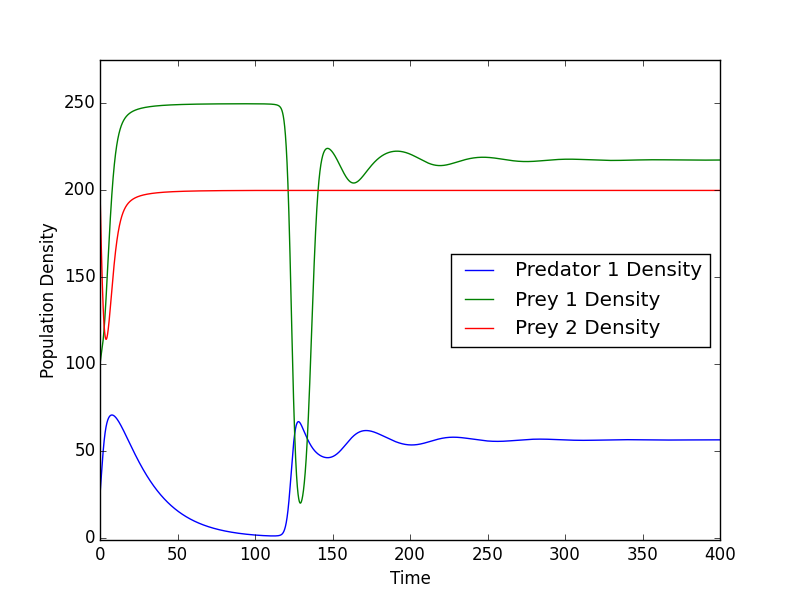
\includegraphics[scale=0.5]{figures/1x2/densities_generalist_to_specialist.png}
\end{frame}
\begin{frame}
	\frametitle{Figures}
	{\bf Generalist Becomes Specialist}
	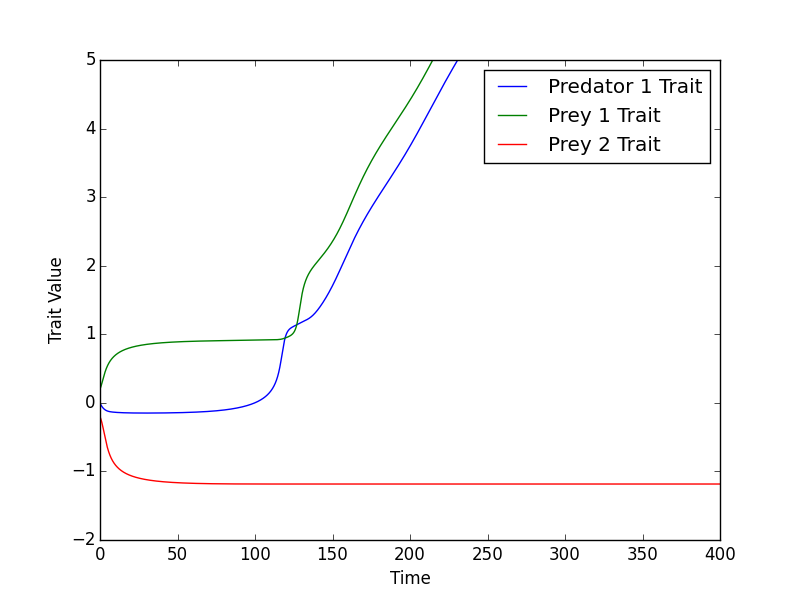
\includegraphics[scale=0.5]{figures/1x2/traits_generalist_to_specialist.png}
\end{frame}
\begin{frame}
	\frametitle{Figures}
	{\bf Unstable Coexistence}
	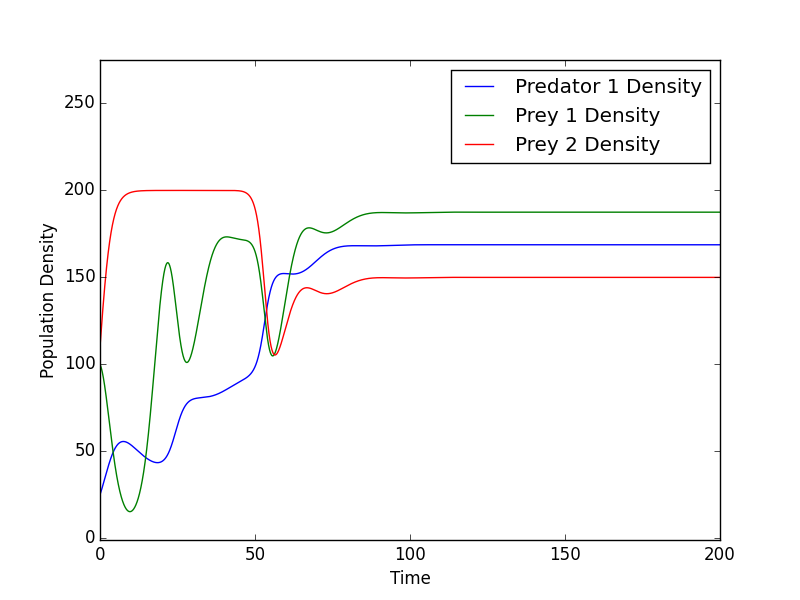
\includegraphics[scale=0.5]{figures/1x2/densities_unstable_coexistence.png}
\end{frame}
\begin{frame}
	\frametitle{Figures}
	{\bf Unstable Coexistence}
	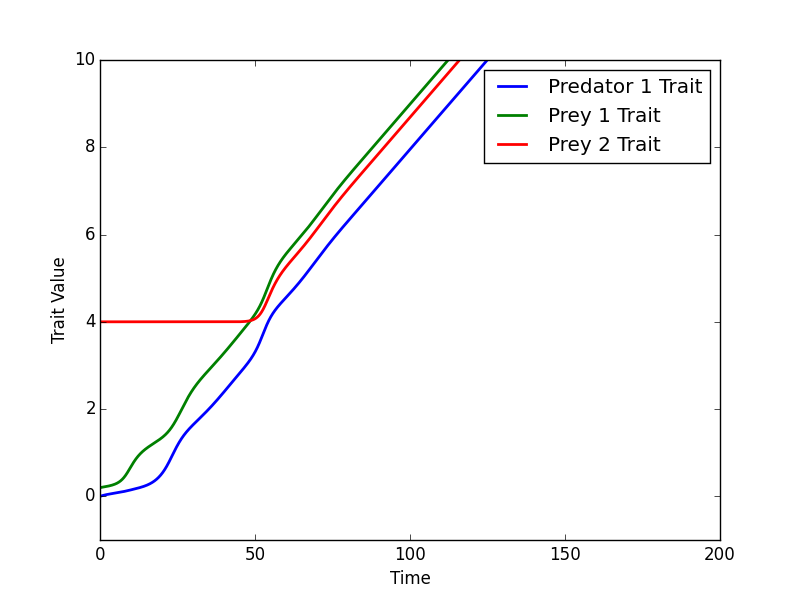
\includegraphics[scale=0.5]{figures/1x2/traits_unstable_coexistence.png}
\end{frame}

\section{Thanks}





\end{document}